\clearpage

\section{Toy MC study of biases in joint oscillation analysis fitter}
\label{app:fitterbias}

A study was performed to check whether the true input oscillation points could be recovered by the joint oscillation analysis fitter 
(equation \ref{eq:chisqtot}). This check was made for various sets of oscillation parameters; each set checked the fitted values of one oscillation 
parameter, while the input values of the other three were fixed to the default values shown in table \ref{tab:defaultvaluesresiduals}. 500 toy MC experiments 
were created for each set with statistical fluctuations. The joint oscillation analysis fitter was run on each toy MC experiment, with systematic parameters 
being allowed to float, and the values returned by the fitter were compared with the true input values. This study was done for both the Run 1+2 POT 
(1.43$\times$10$^{20}$) and for the estimated final POT (7$\times$10$^{21}$).

\begin{table}[h]
\centering
\begin{tabular}{|c|c|}
\hline
Parameter & Value \\
\hline \hline
$\sin^{2}2\theta_{23} $ &  0.96 \\
$\sin^{2}\theta_{23} $ & 0.64\\
$\sin^{2}2\theta_{13} $ &  0.09 \\
$\sin^{2}\theta_{13} $ & 0.02\\
$|\Delta m_{32}^{2}|$ & 2.4$\times$10$^{-3}$ eV$^{2}$/c$^{4}$ \\
$\delta_{CP}$ & 0.0 \\
\hline
\end{tabular}
\caption{Default input values used for each oscillation parameter in the toy MC experiments created for the study of fitter residuals (fitted value - true input value)}
\label{tab:defaultvaluesresiduals}
\end{table}

In figure \ref{fig:res2theta}, the fitter residuals (fitted value - true input value) are shown for the estimated final POT (7$\times$10$^{21}$) for 
$\sin^{2}2\theta_{23}$ (top left), $|\Delta m_{32}^{2}|$ (top right), $\sin^{2}2\theta_{13}$ (bottom left) and $\delta_{CP}$ (bottom right). From this figure, 
it is apparent that there are no biases in the fitted values of $\sin^{2}2\theta_{23}$, $|\Delta m_{32}^{2}|$ and $\sin^{2}2\theta_{13}$ (the peak at +0.01 for 
an input value of 0.99 for $\sin^{2}2\theta_{23}$ is due to pile-up at the physical boundary). However the residuals of $\delta_{CP}$ show that the fitter tends 
to return values of 0 or $\pm \pi$ for this parameter; this bias in fitting $\delta_{CP}$ has been studied in more detail, and the results are shown in 
Appendix \ref{subsec:deltaCP}. 

\begin{figure}[htbp]
\begin{center}
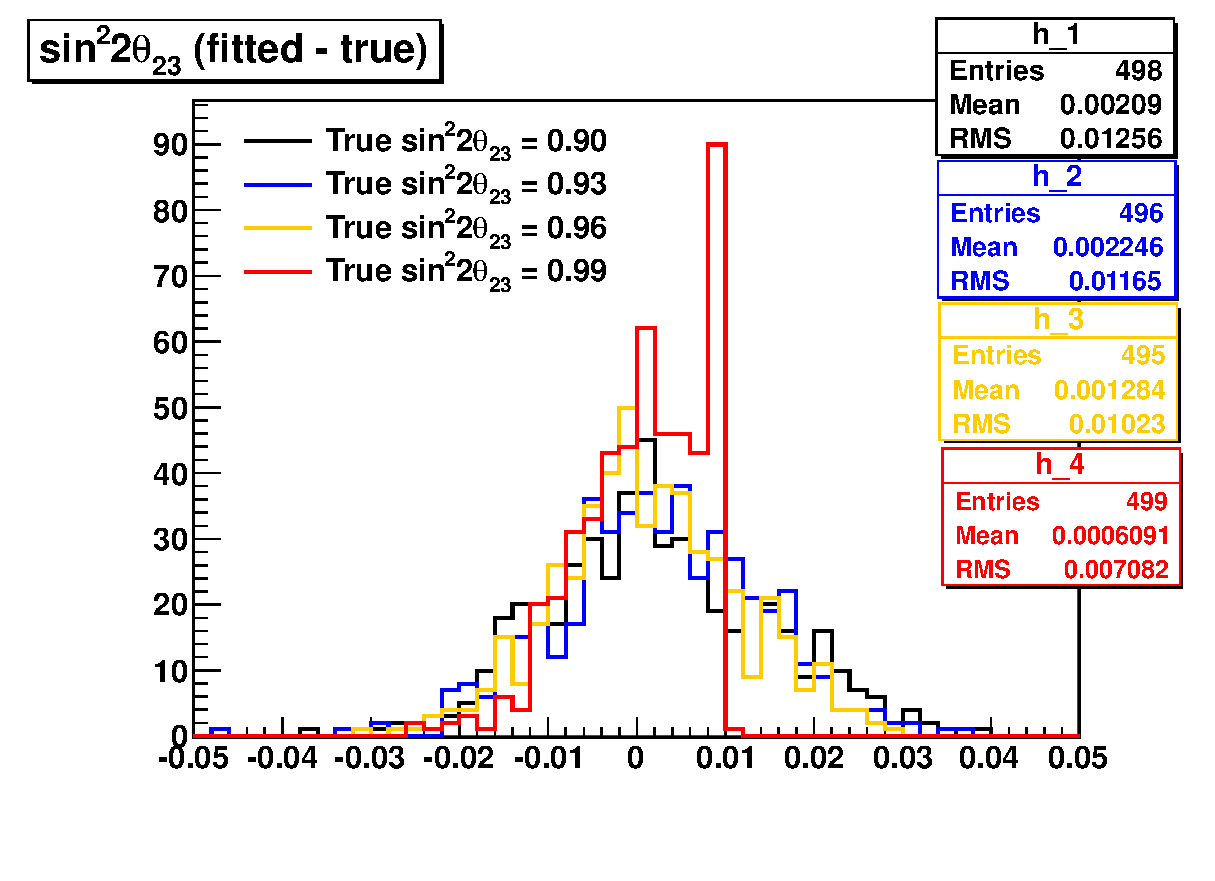
\includegraphics[width=0.5\textwidth]{images/validation/ResidualsSinsq2Theta23.eps}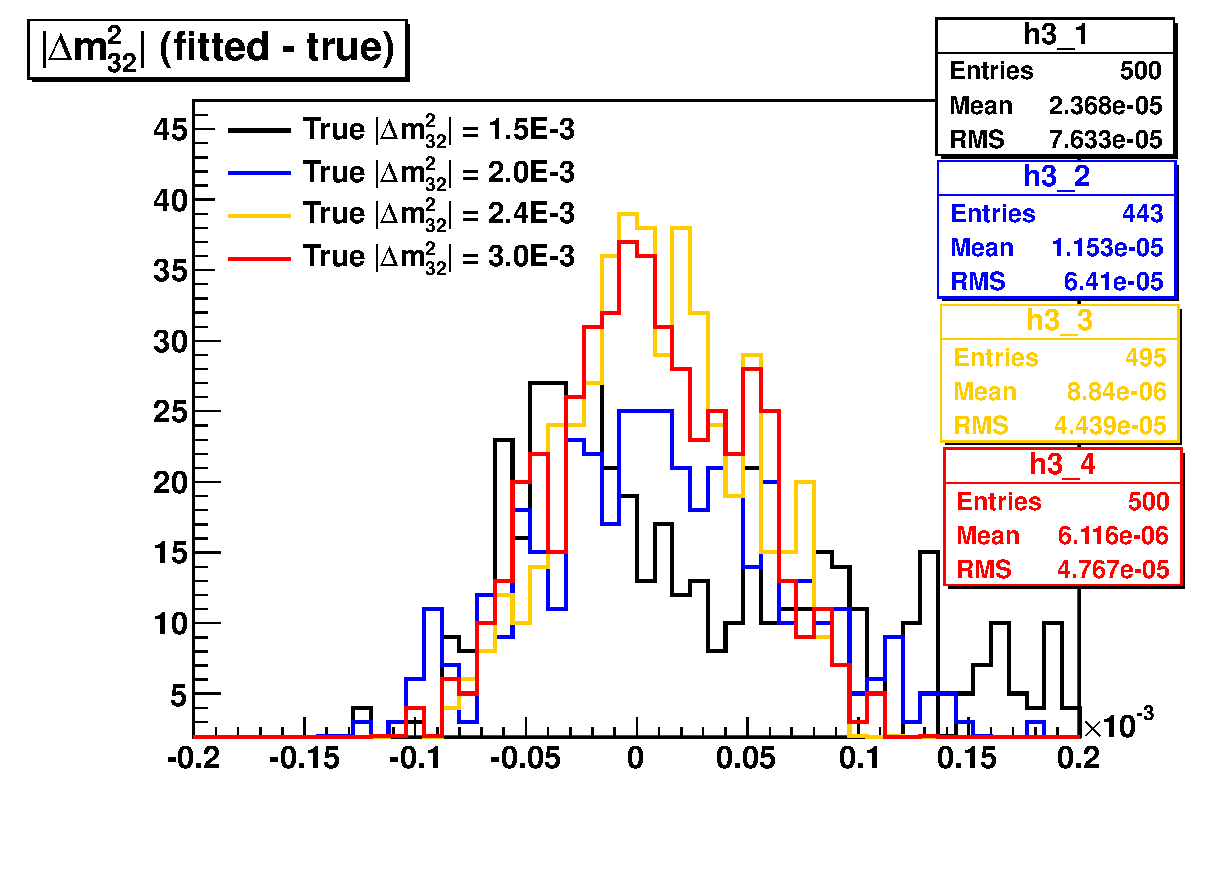
\includegraphics[width=0.5\textwidth]{images/validation/ResidualsDmsq23.eps}
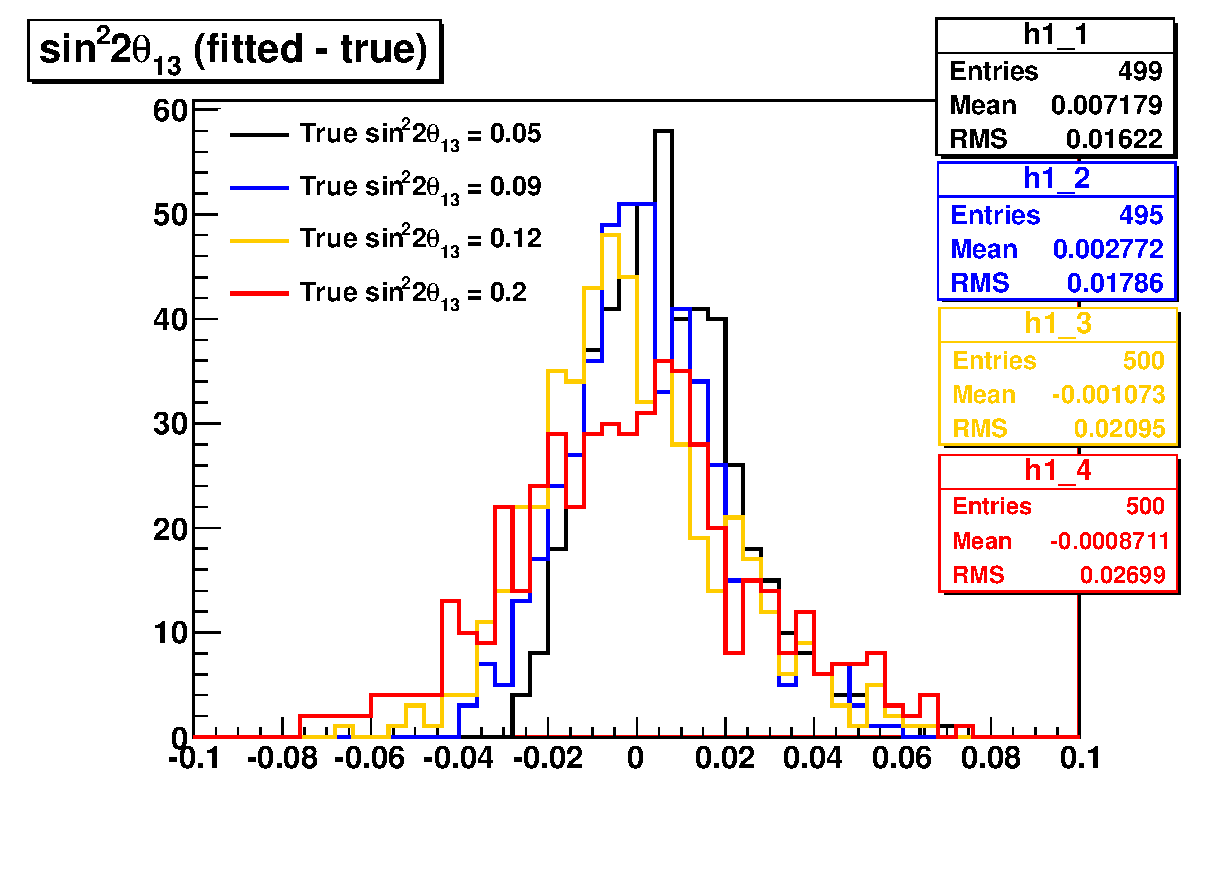
\includegraphics[width=0.5\textwidth]{images/validation/ResidualsSinsq2Theta13.eps}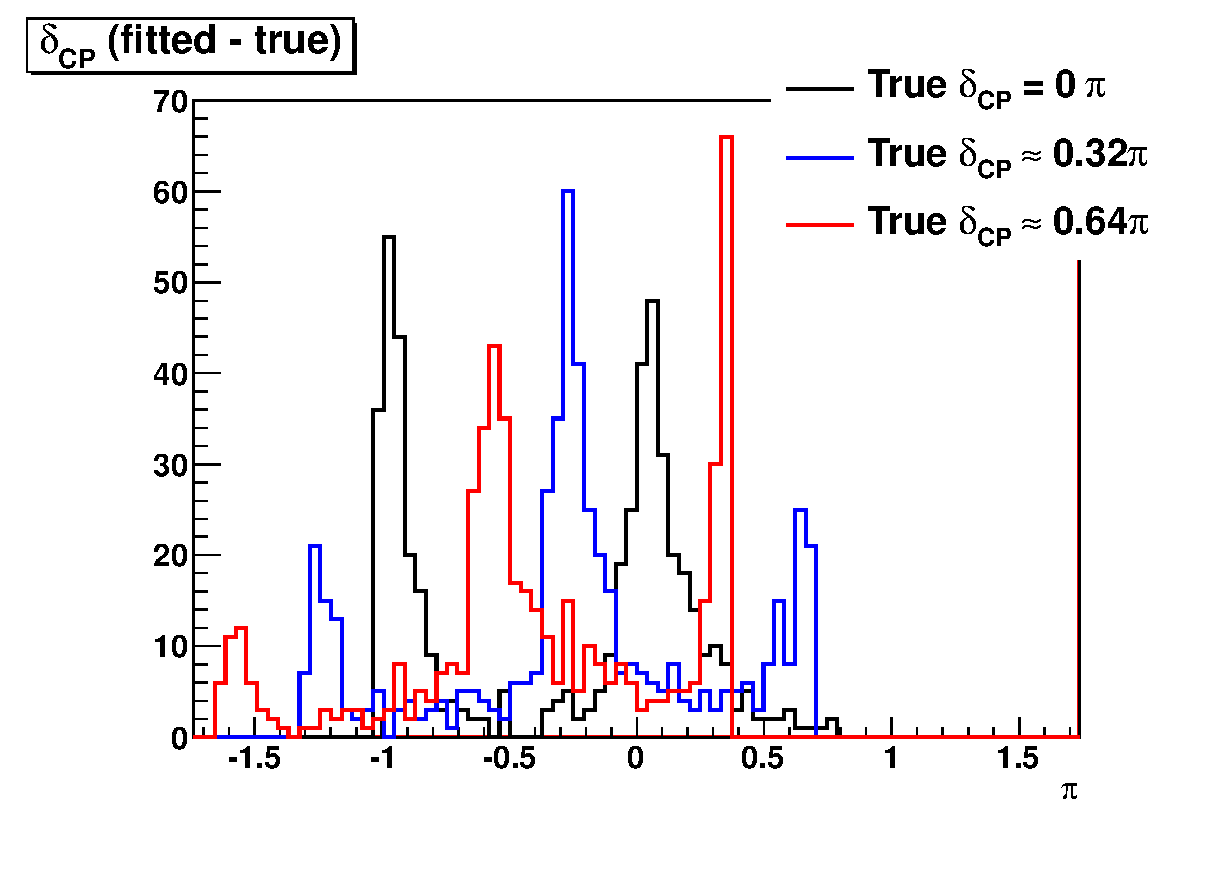
\includegraphics[width=0.5\textwidth]{images/validation/ResidualsDeltaCP.eps}
\caption{Fitter residuals (fitted value - true input value) for $\sin^{2}2\theta_{23}$, $|\Delta m_{32}^{2}|$, $\sin^{2}2\theta_{13}$ and $\delta_{CP}$ for 
the estimated final POT (7$\times$10$^{21}$).}
\label{fig:res2theta}
\end{center}
\end{figure}

The fitter residuals are also shown for the Run 1+2 POT (1.43$\times$10$^{20}$) in figures \ref{fig:residuals2thetacurrtheta23} and \ref{fig:res2thetacurroth}. The 
pile-up in the fitted values of $\sin^{2}2\theta_{23}$ at the physical boundary is more pronounced with less POT as shown in figure \ref{fig:residuals2thetacurrtheta23}; 
this is due to the wider distribution of the fitted values with less statistics. There is again no bias in the fitted values of $|\Delta m_{32}^{2}|$ and $\sin^{2}2\theta_{13}$, 
and the distribution of fitted values of $\delta_{CP}$ is similar to that in figure \ref{fig:res2theta}.

\begin{figure}[htbp]
\begin{center}
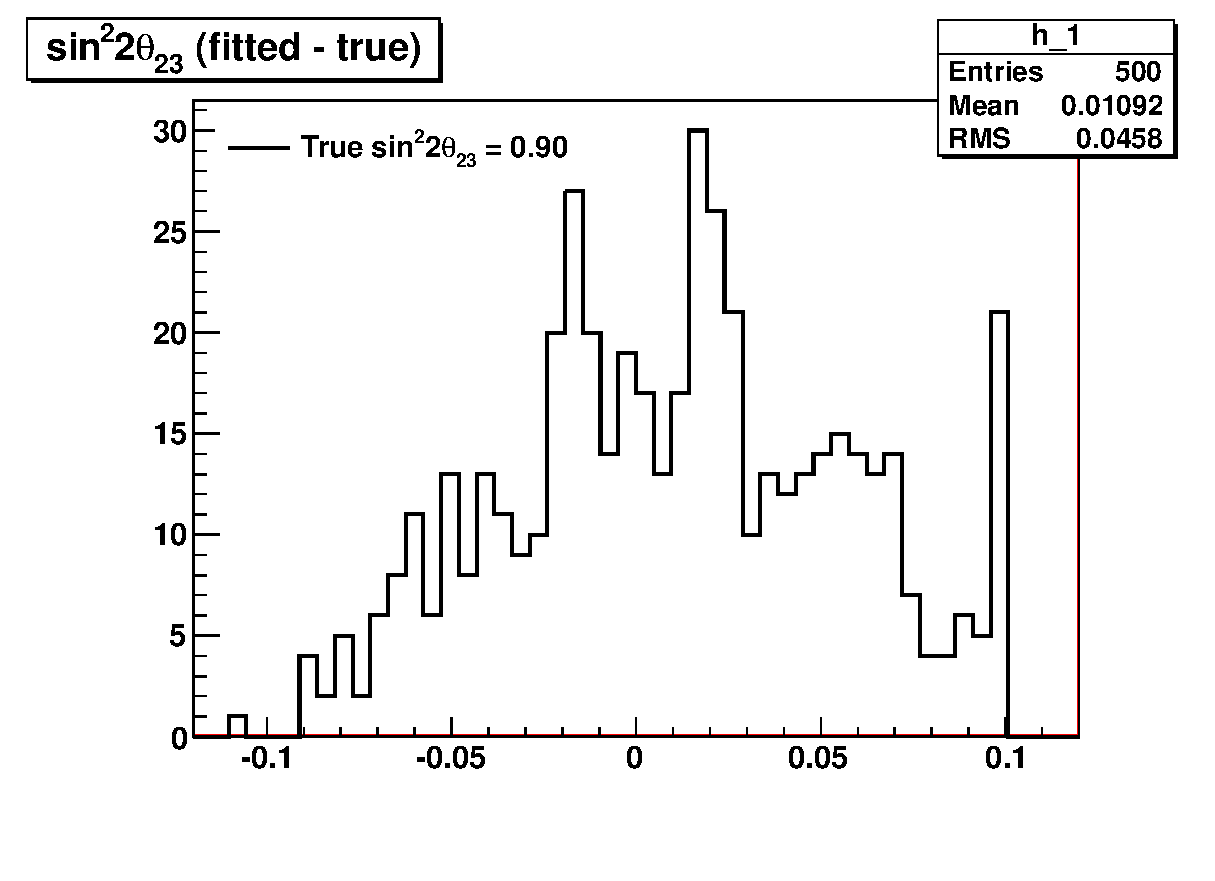
\includegraphics[width=0.5\textwidth]{images/validation/ResidualsSinsq2Theta23Current1.eps}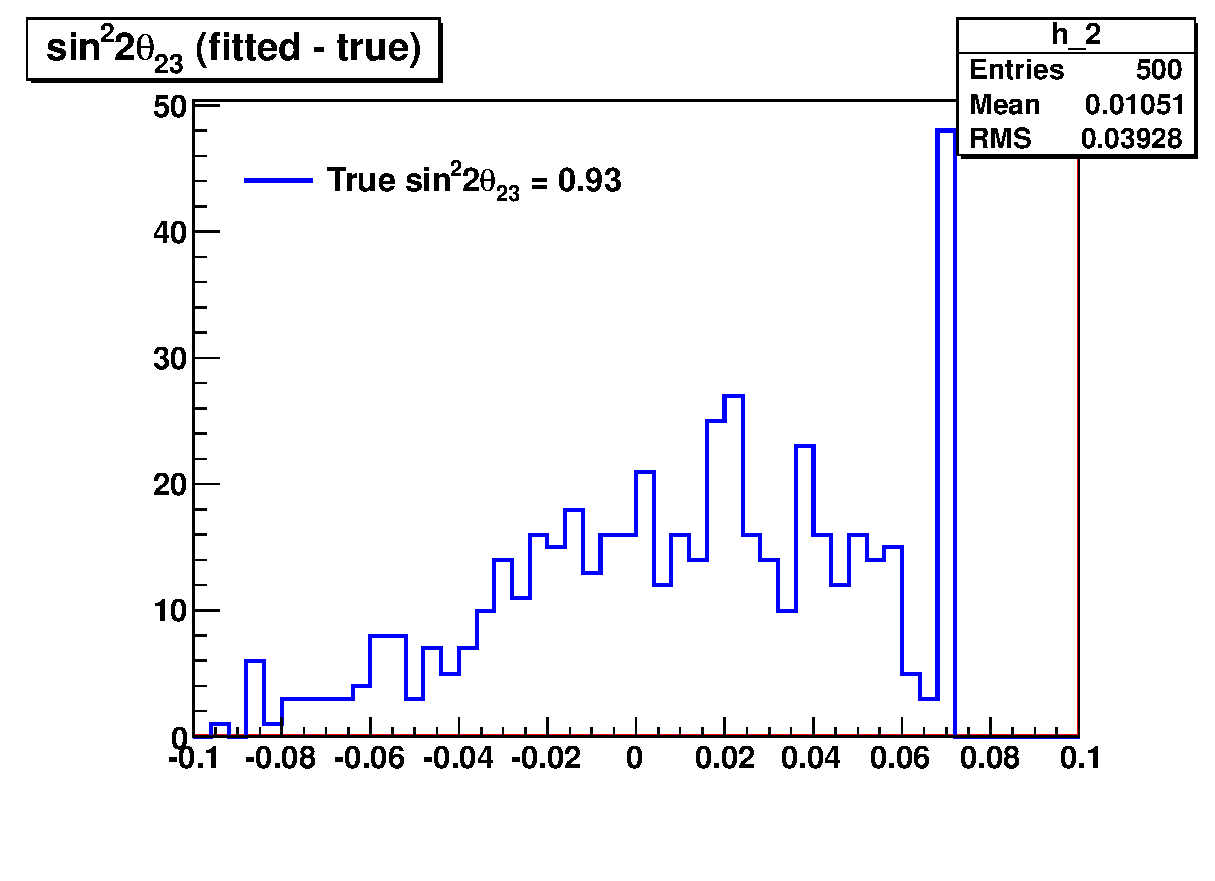
\includegraphics[width=0.5\textwidth]{images/validation/ResidualsSinsq2Theta23Current2.eps}
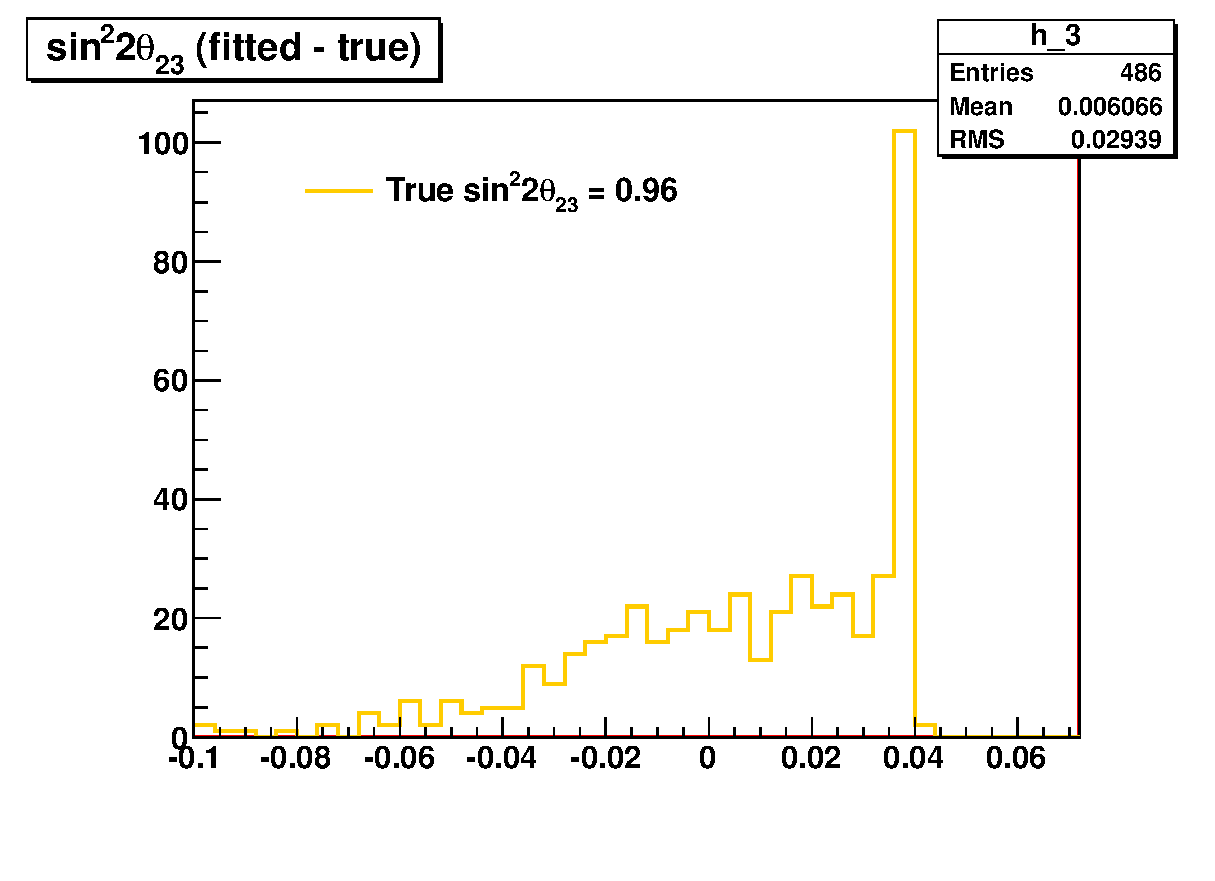
\includegraphics[width=0.5\textwidth]{images/validation/ResidualsSinsq2Theta23Current3.eps}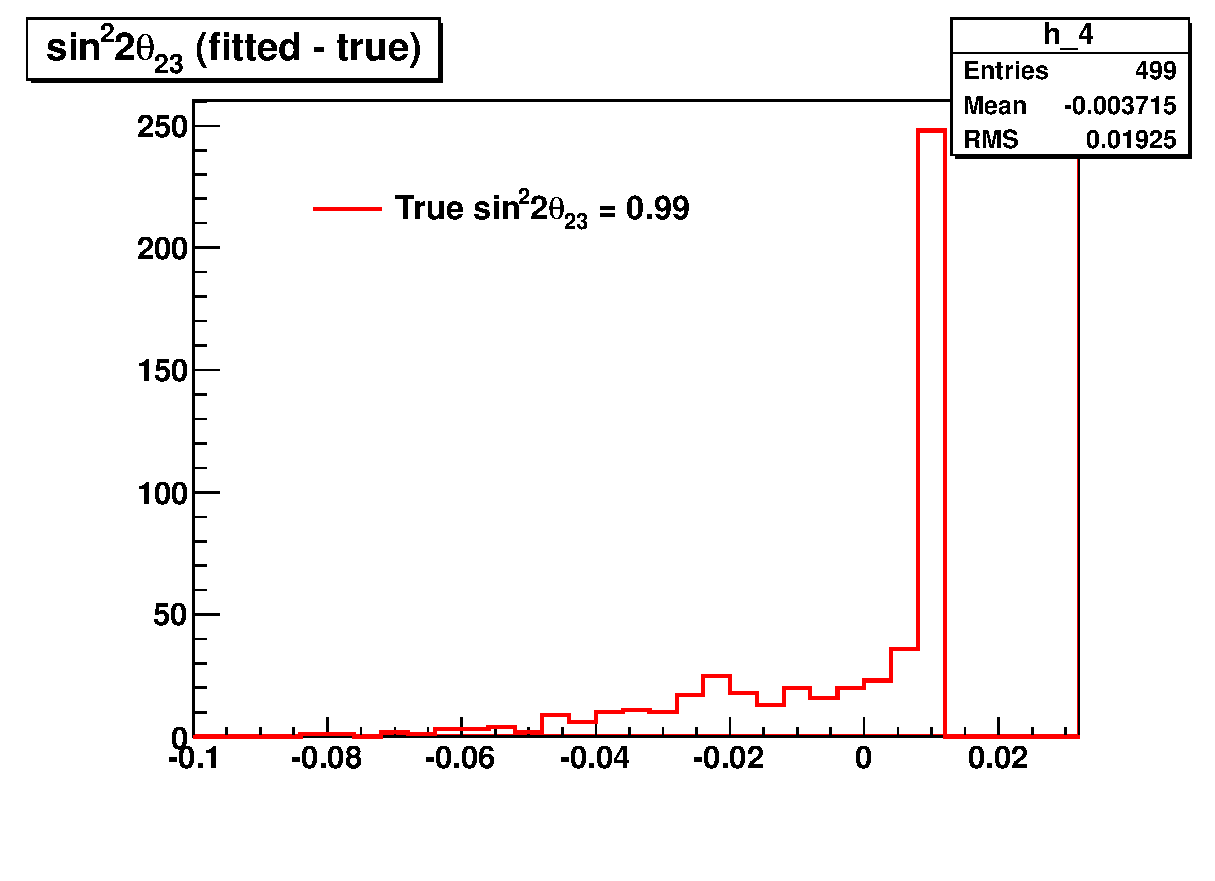
\includegraphics[width=0.5\textwidth]{images/validation/ResidualsSinsq2Theta23Current4.eps}
\caption{Fitter residuals (fitted value - true input value) for $\sin^{2}2\theta_{23}$ for the Run 1+2 POT (1.43$\times$10$^{20}$).}
\label{fig:residuals2thetacurrtheta23}
\end{center}
\end{figure}


\begin{figure}[htbp]
\begin{center}
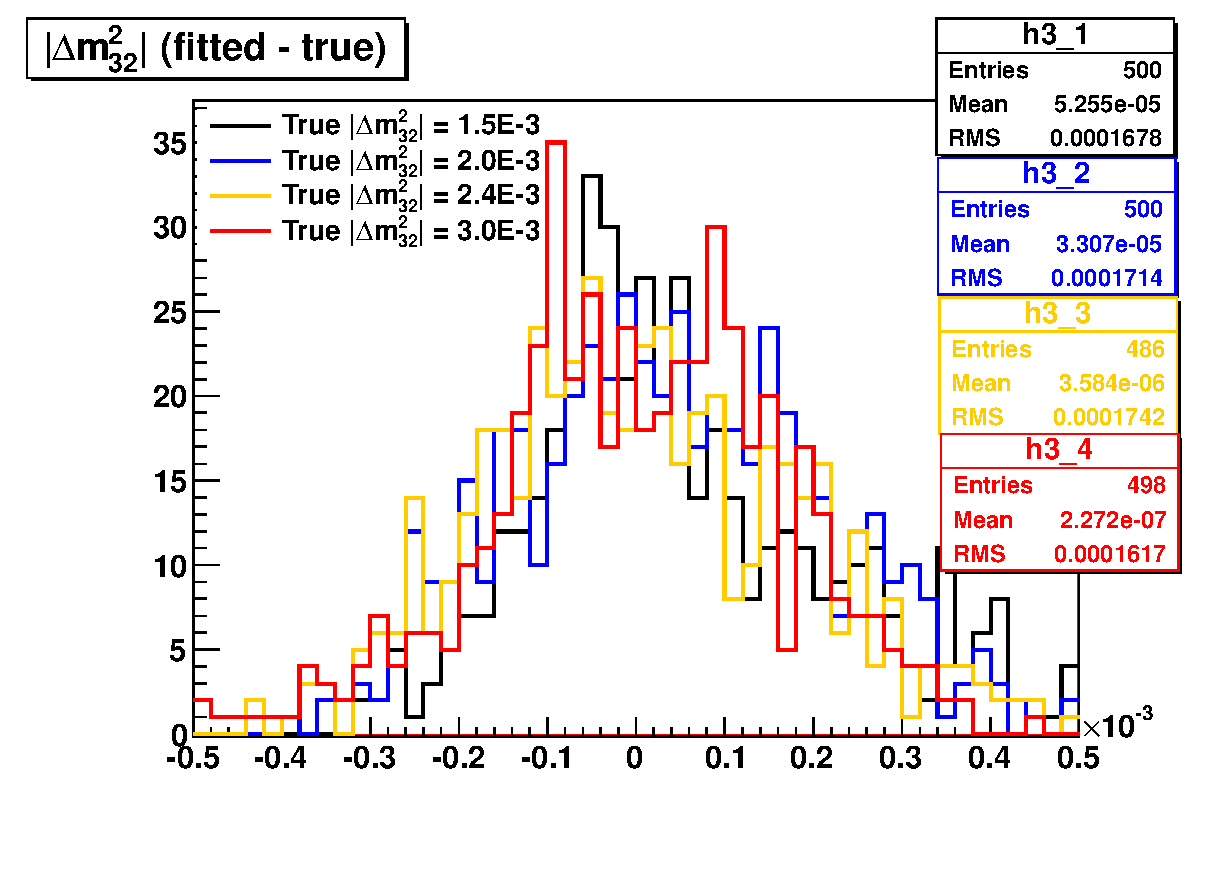
\includegraphics[width=0.5\textwidth]{images/validation/ResidualsSinsq2Dmsq23Current.eps}
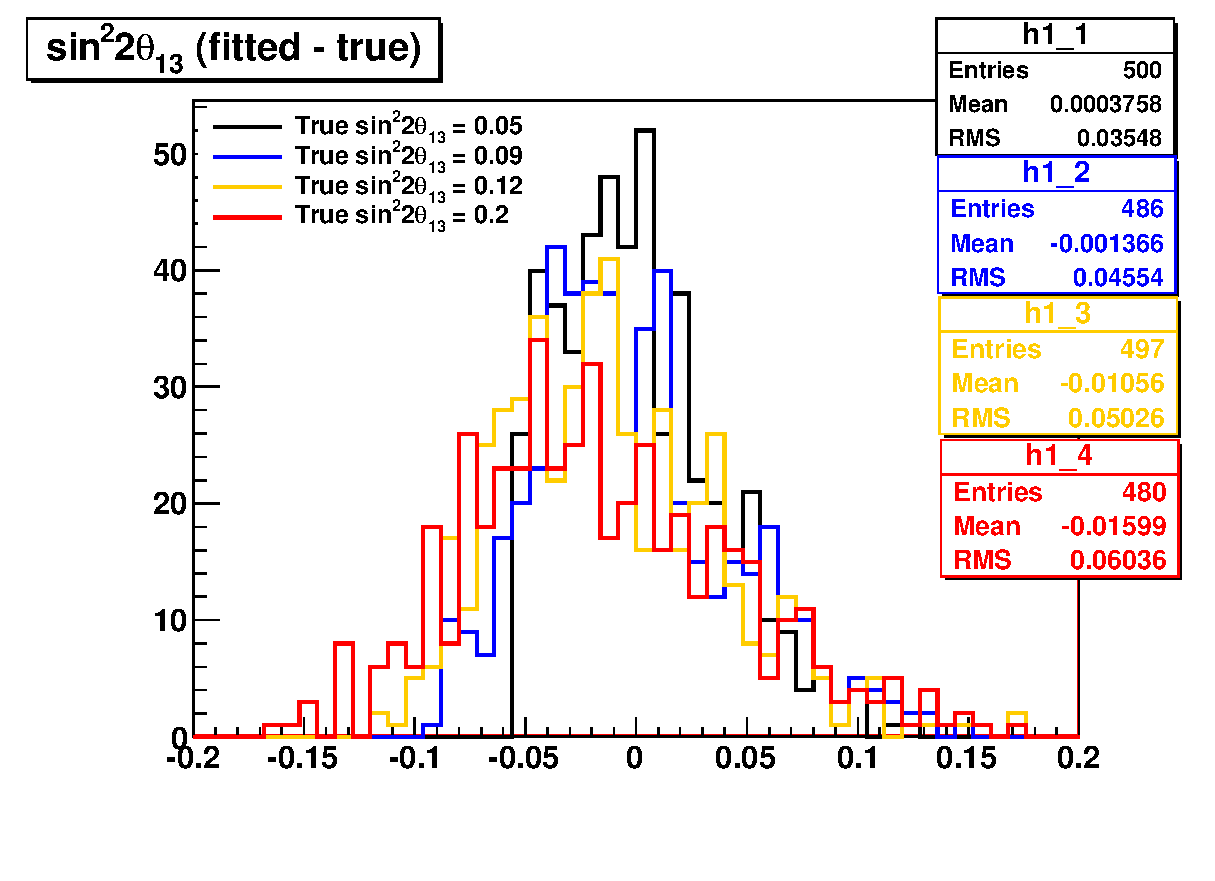
\includegraphics[width=0.5\textwidth]{images/validation/ResidualsSinsq2Theta13Current.eps}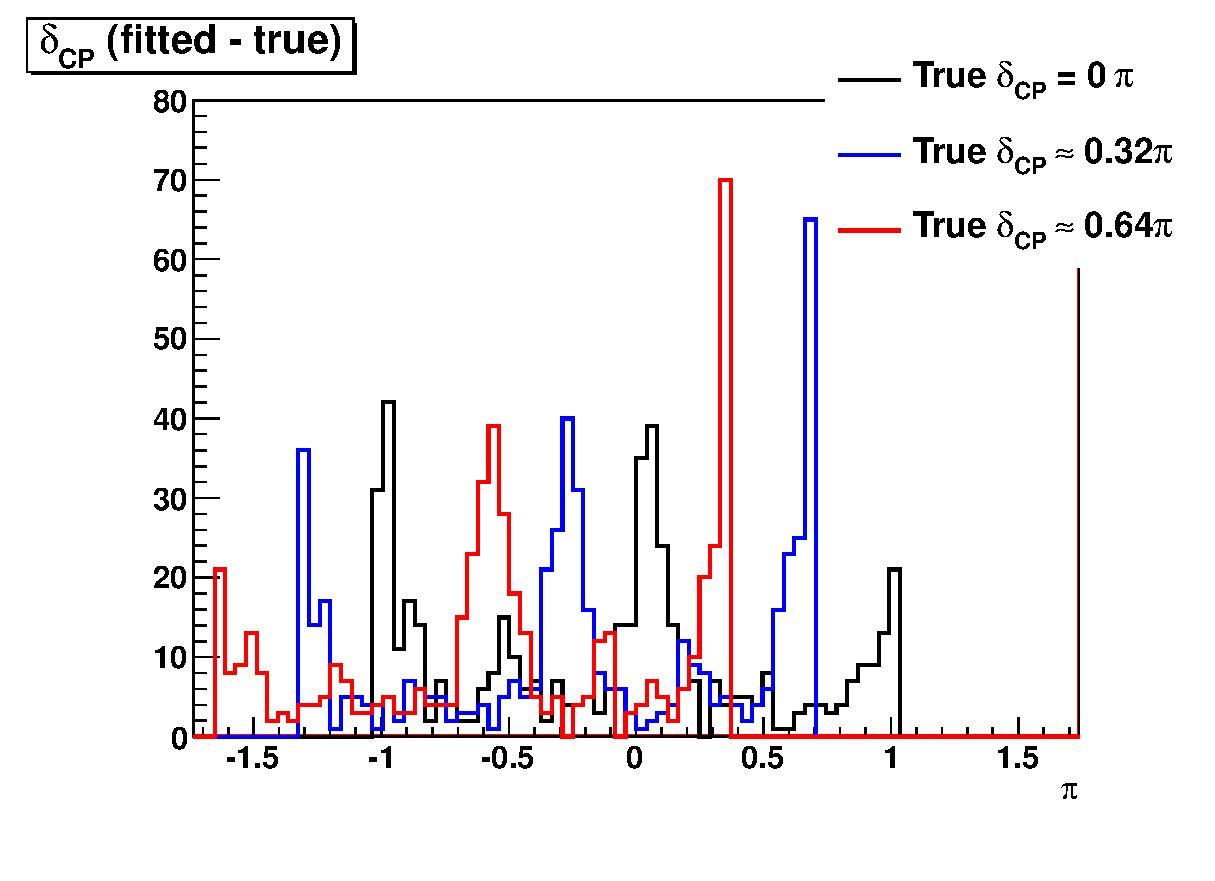
\includegraphics[width=0.5\textwidth]{images/validation/ResidualsDeltaCPCurrent.eps}
\caption{Fitter residuals (fitted value - true input value) for $|\Delta m^{2}_{32}|$, $\sin^{2}2\theta_{13}$ and $\delta_{CP}$ for the Run 1+2 POT (1.43$\times$10$^{20}$).}
\label{fig:res2thetacurroth}
\end{center}
\end{figure}

The fitter residuals were also checked for the mixing angles in the form $\sin^{2}\theta_{ij}$ for the estimated final POT (7$\times$10$^{21}$). For 
$\sin^{2}\theta_{23}$, the fit was made twice with the initial value in each octant as described in section \ref{sec:initvalues_range}; this was done due to the 
fitter tending to return a fitted value in the same octant as the initial value. Despite using two fits in this way, the residuals for $\sin^{2}\theta_{23}$ still 
have two peaks: one peak is centered on zero (for fitted values in the correct octant) while the other is biased (for fitted values in the mirror octant), and this 
is shown in figure \ref{fig:residualstheta23}. The presence of the two peaks can be explained by the fitted values of $\sin^{2}\theta_{13}$: if the residual of 
$\sin^{2}\theta_{23}$ is small, the residual of $\sin^{2}\theta_{13}$ is also small, but, when the fitted value of $\sin^{2}\theta_{23}$ is in the mirror octant, 
the fitter compensates by returning an incorrect fitted value of $\sin^{2}\theta_{13}$. This behaviour of the fitter is clearly shown by the two distinct 
distributions of residuals of these two mixing angles in figure \ref{fig:residualstheta13theta23}. The pile-up at maximal $\sin^{2}\theta_{23}$ is also seen when 
the true input value is near the centre of symmetry, for example in the left plot of figure \ref{fig:residualstheta23}.
 
\begin{figure}[htbp]
\begin{center}
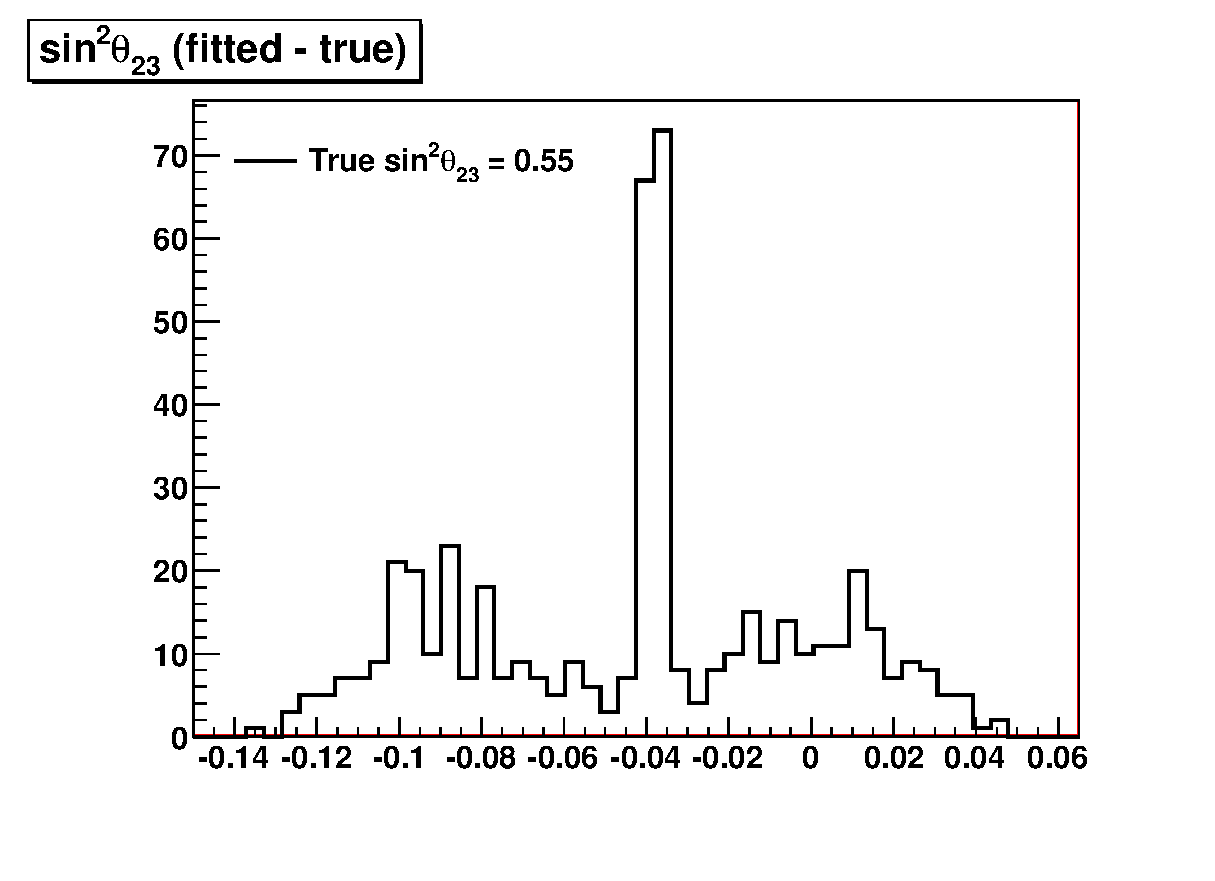
\includegraphics[width=0.35\textwidth]{images/validation/ResidualsSinsqTheta23Set1.eps}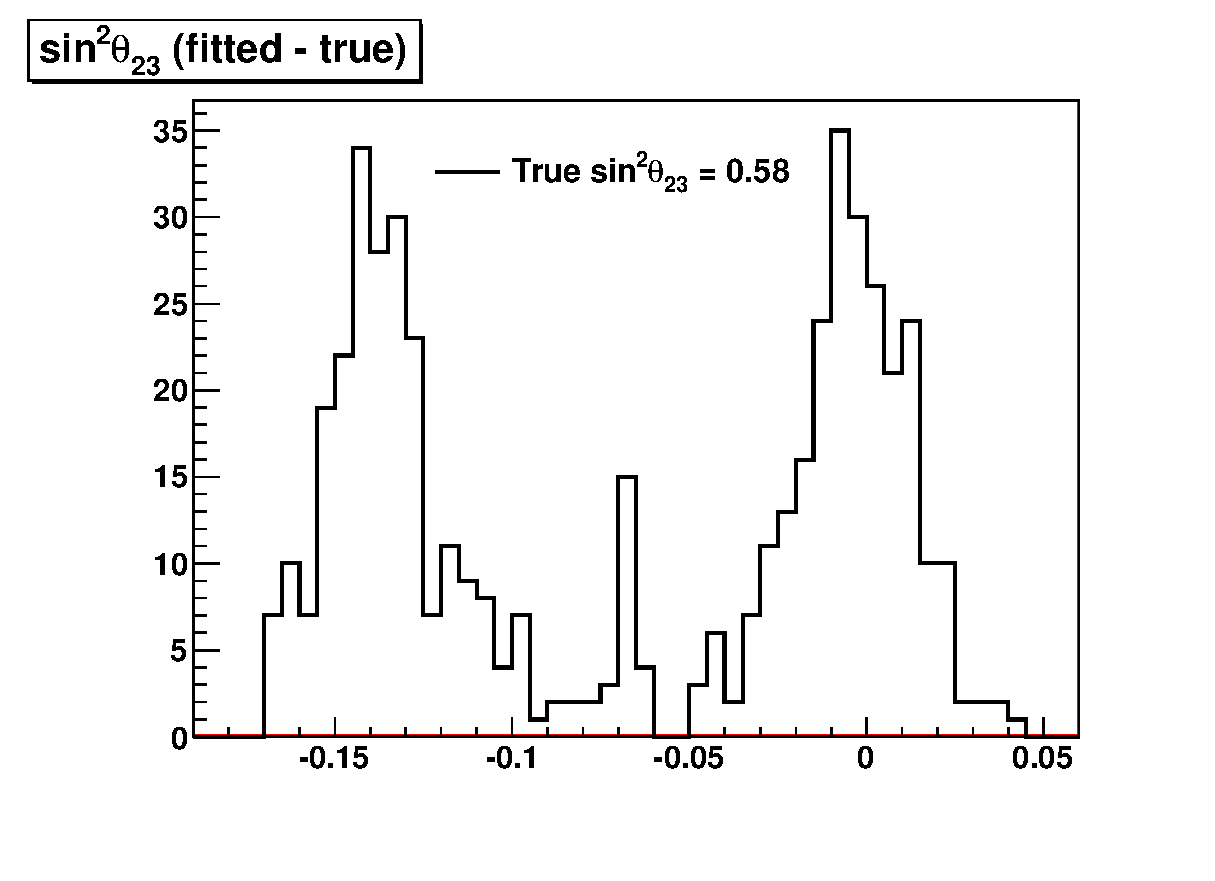
\includegraphics[width=0.35\textwidth]{images/validation/ResidualsSinsqTheta23Set2.eps}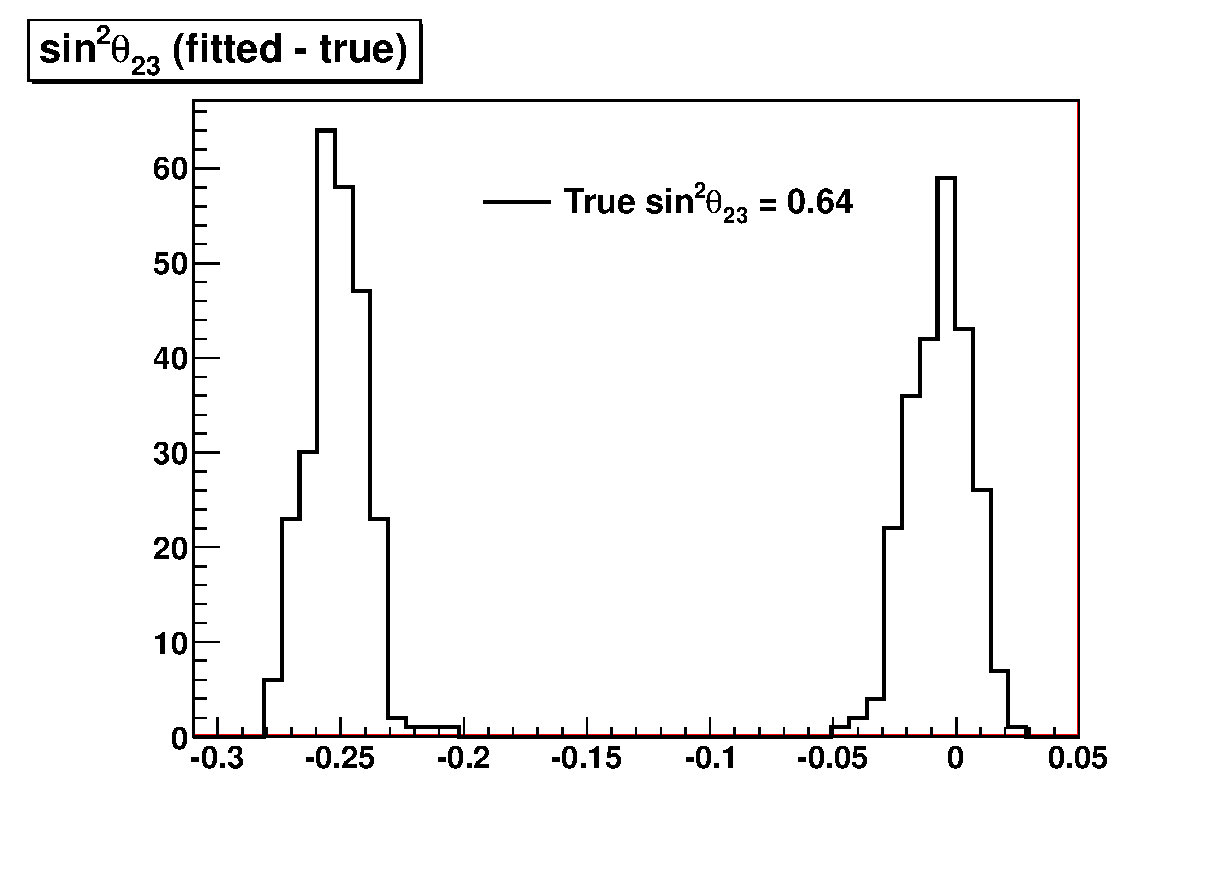
\includegraphics[width=0.35\textwidth]{images/validation/ResidualsSinsqTheta23Set3.eps}
\caption{Fitter residuals (fitted value - true input value) for $\sin^{2}\theta_{23}$ for the estimated final POT (7$\times$10$^{21}$).}
\label{fig:residualstheta23}
\end{center}
\end{figure}

\begin{figure}[htbp]
\begin{center}
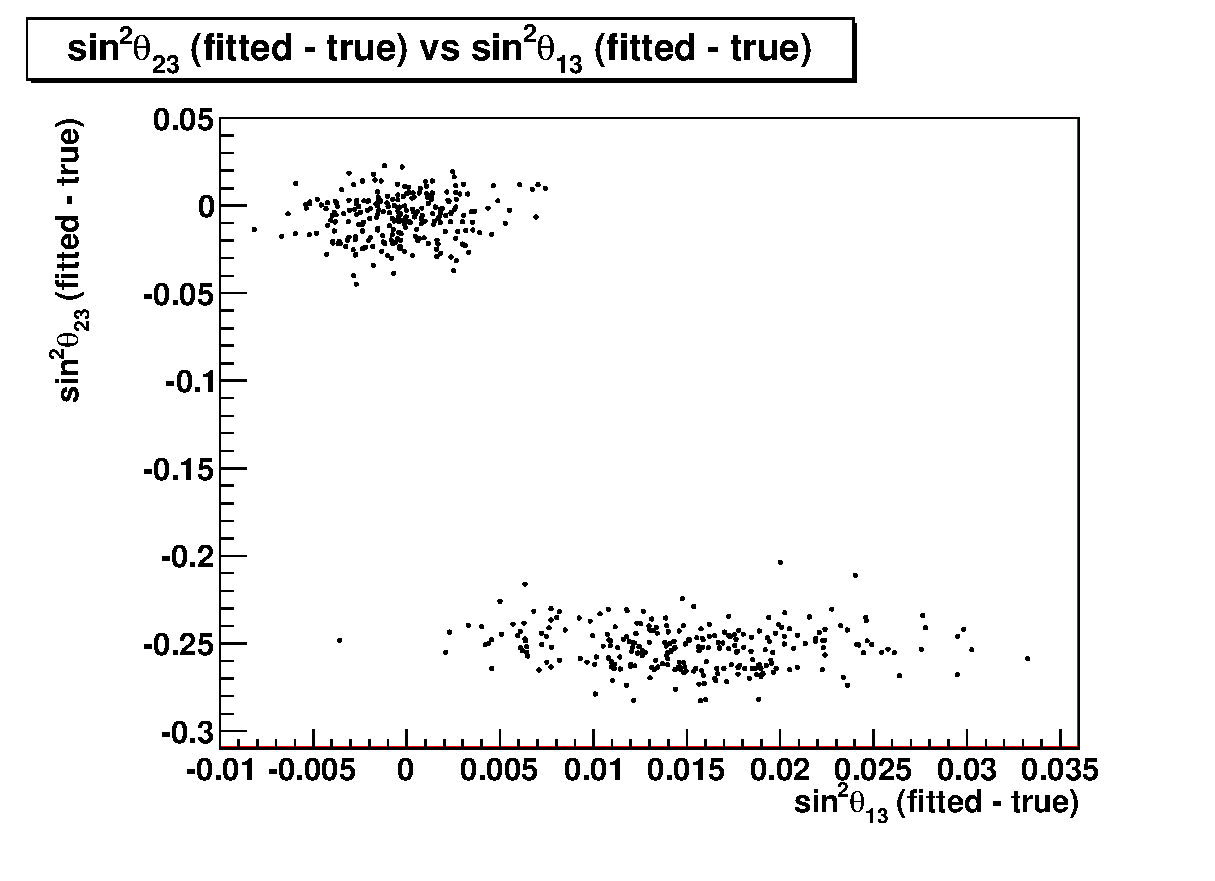
\includegraphics[width=0.7\textwidth]{images/validation/ExampleTheta23Theta13OctantsSet4.eps}
\caption{Fitter residuals (fitted value - true input value) for $\sin^{2}\theta_{23}$ against residuals for $\sin^{2}\theta_{13}$ for the estimated final POT 
(7$\times$10$^{21}$); the true input value of $\sin^{2}\theta_{23}$ is 0.64.}
\label{fig:residualstheta13theta23}
\end{center}
\end{figure}
An attempt was made to overcome the problem of the incorrect fitting of $\sin^{2}\theta_{23}$ by constraining the fitted value of $\sin^{2}\theta_{13}$. This was done 
through the penalty term in equation \ref{eq:chisqtot}, setting the mean of $\sin^{2}\theta_{13}$ to 0.09 (its true input value) and its error to 20\%. With this constraint, 
the fitted values of $\sin^{2}\theta_{23}$ were nearly all in the correct octant, and the fitter residuals were nearly all in a single peak centered on zero (see 
figure \ref{fig:residualstheta13theta23const}, right plot); the fitter residuals of $\sin^{2}\theta_{13}$ were also all in a single peak centered on zero (see 
figure \ref{fig:residualstheta13const}, right plot). 

\begin{figure}[htbp]
\begin{center}
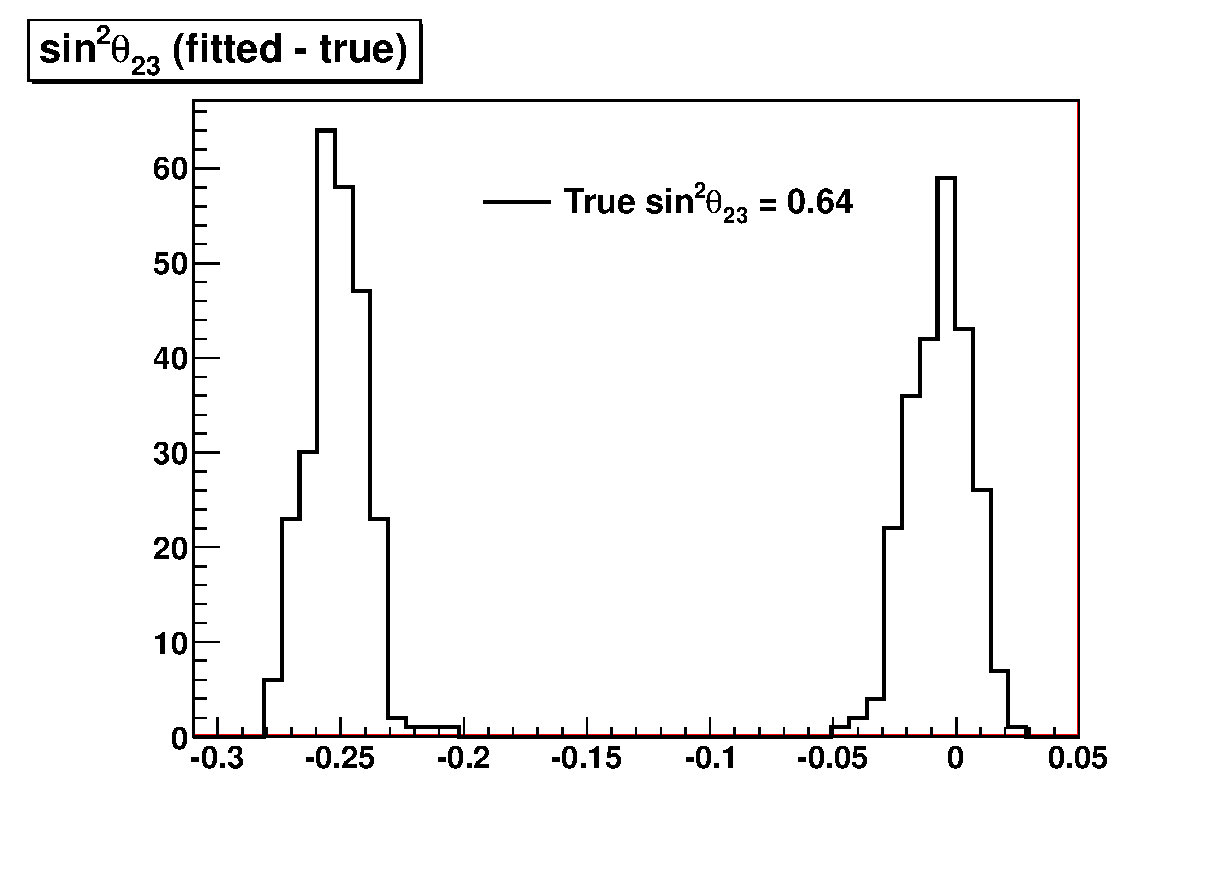
\includegraphics[width=0.5\textwidth]{images/validation/ResidualsSinsqTheta23Set3.eps}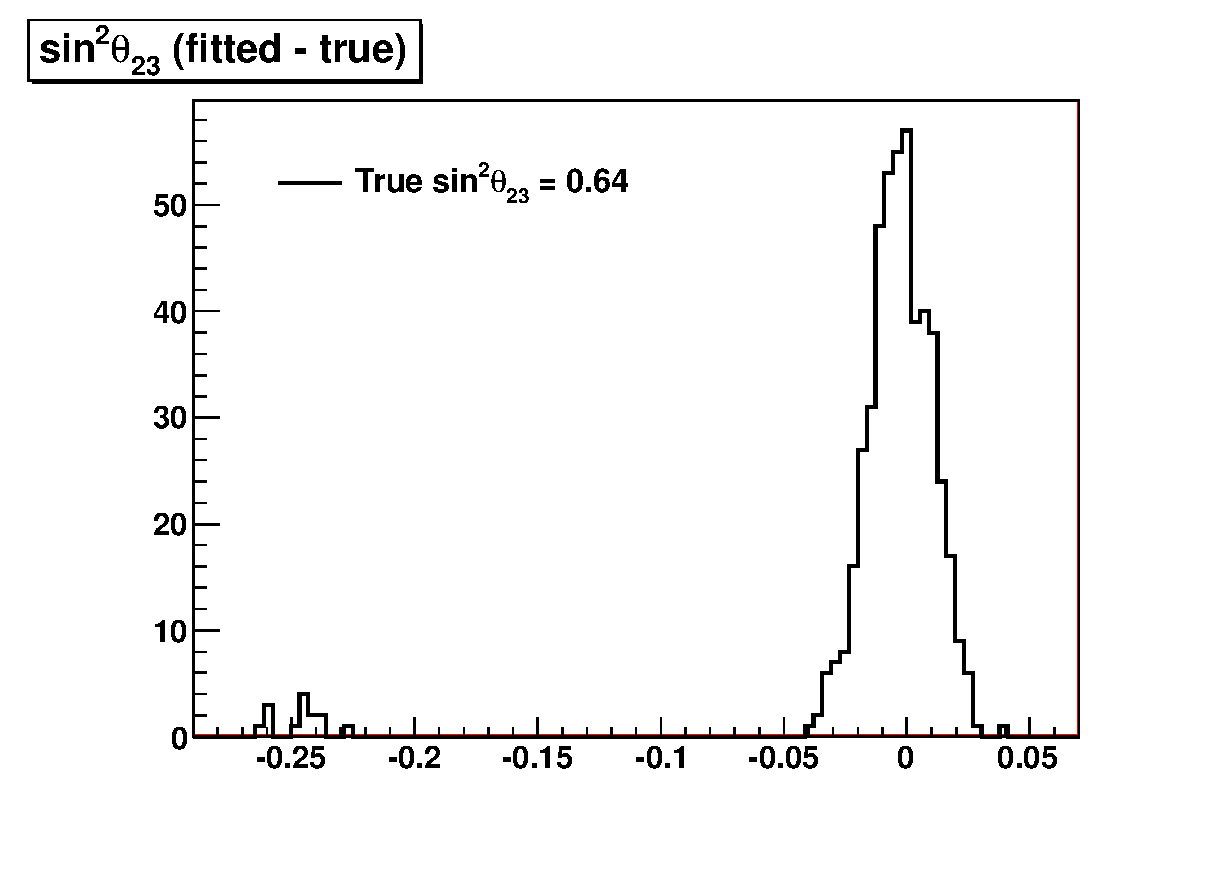
\includegraphics[width=0.5\textwidth]{images/validation/ResidualsSinsqTheta23Set3Constrain.eps}
\caption{Example of the effect of constraining the fitted value of $\sin^{2}\theta_{13}$ to have a mean of 0.09 (its true input value) and a 20\% error on the 
distribution of fitter residuals for $\sin^{2}\theta_{23}$ for the estimated final POT (7$\times$10$^{21}$). Without the constraint the residuals have two peaks, 
one in each octant (left), but with the constraint the peak in the incorrect octant nearly disappears (right). The true input value of $\sin^{2}\theta_{23}$ is 0.64.}
\label{fig:residualstheta13theta23const}
\end{center}
\end{figure}

\begin{figure}[htbp]
\begin{center}
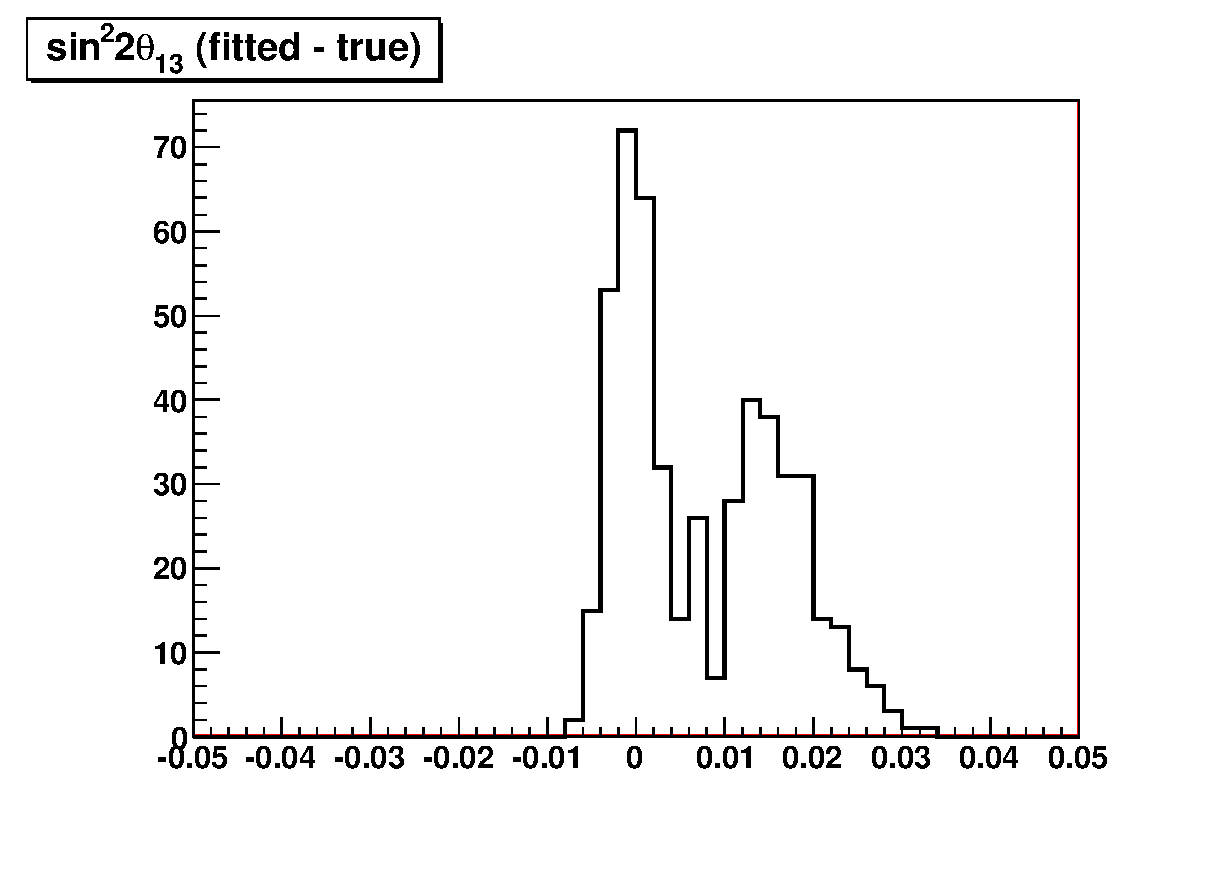
\includegraphics[width=0.5\textwidth]{images/validation/ResidualsSinsqTheta13BeforeConstraining.eps}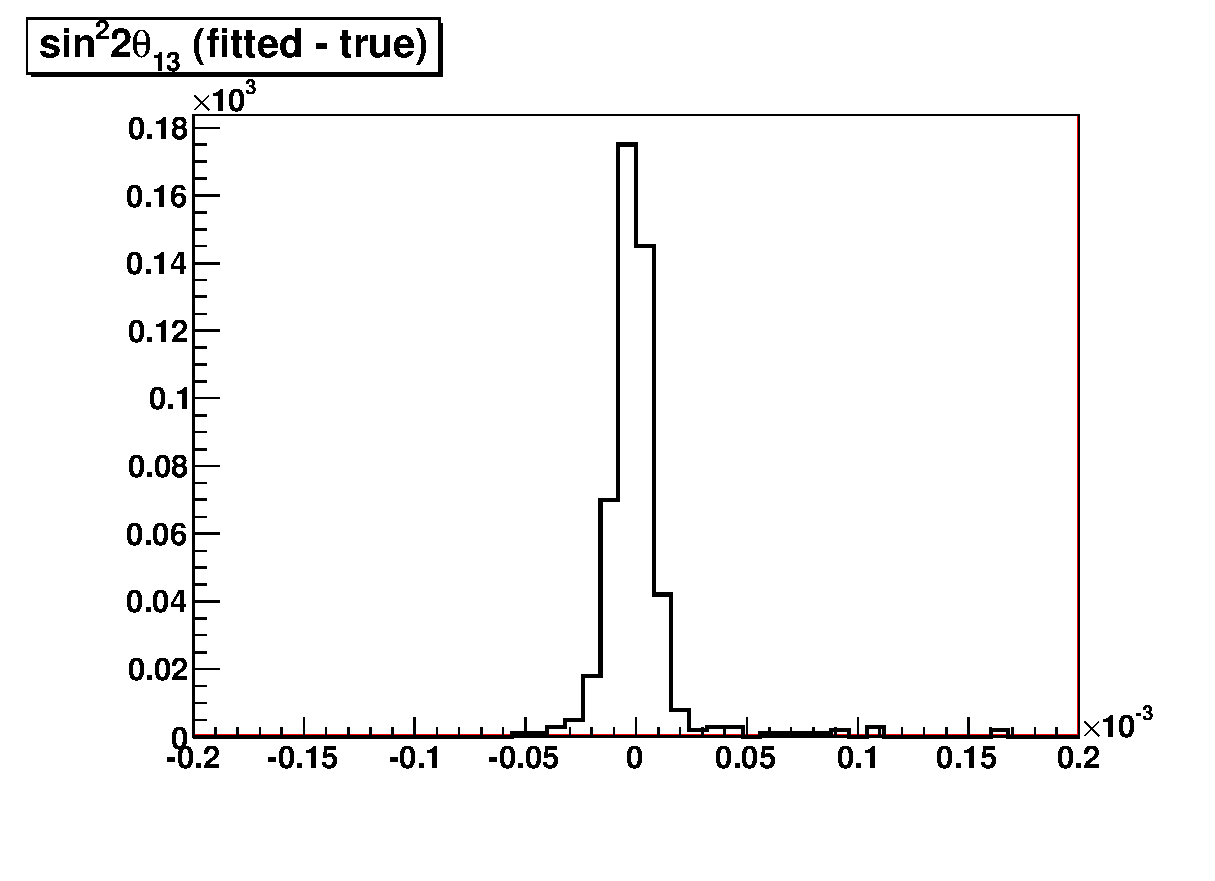
\includegraphics[width=0.5\textwidth]{images/validation/ResidualsSinsqTheta13AfterConstraining.eps}
\caption{Example of the effect of constraining the fitted value of $\sin^{2}\theta_{13}$ to have a mean of 0.09 (its true input value) and a 20\% error on the
distribution of fitter residuals for $\sin^{2}\theta_{13}$ for the estimated final POT (7$\times$10$^{21}$). Without the constraint the residuals have two peaks 
(left), but with the constraint the residuals are all in a single peak centered on zero (right).}
\label{fig:residualstheta13const}
\end{center}
\end{figure}
A study was also made of the effect of constraining the fitted value of $\sin^{2}\theta_{13}$ on the best-fit one $\mu$-like ring spectrum and the best-fit numbers of one 
$\mu$-like ring and one e-like ring events. In figure \ref{fig:rdistributionconst}, the best-fit reconstructed energy spectrum of one $\mu$-like ring events in the first 
octant is shown for an example toy experiment with a true input value of $\sin^{2}\theta_{23}$ = 0.64 both with and without the constraint on the fitted value of 
$\sin^{2}\theta_{13}$. The ratio of the best-fit spectrum in the first octant with the constraint to that without the constraint is also shown; applying the constraint 
changes the spectrum by up to 1\%, with less events at the oscillation maximum and more events immediately above and below it. The best-fit numbers of one $\mu$-like ring 
and one e-like ring events with and without the constraint on $\sin^{2}\theta_{13}$ are also given in table \ref{tab:effconst}; this shows that the constraint can change 
the best-fit numbers of events since, in the example, the best-fit number of one $\mu$-like ring events is increased and the best-fit number of one e-like ring events is 
reduced.
 
\begin{figure}[htbp]
\begin{center}
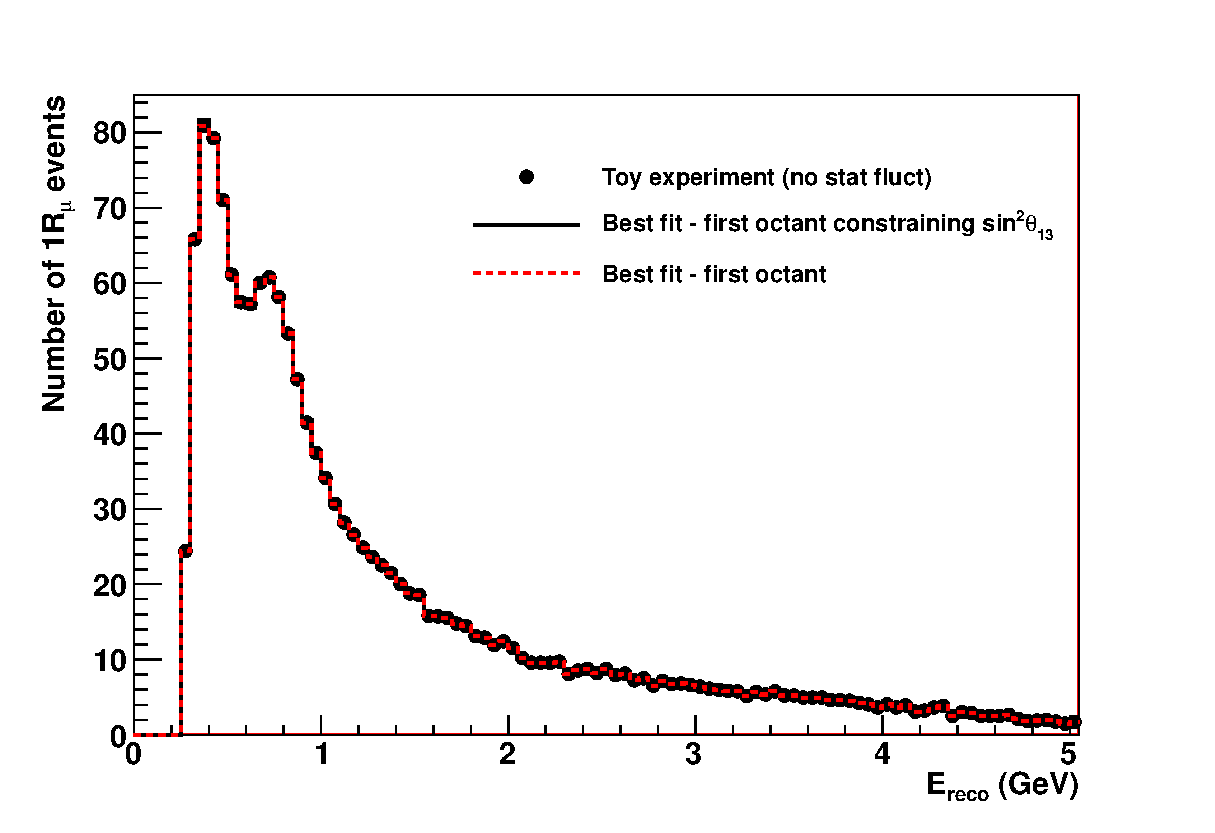
\includegraphics[width=0.5\textwidth]{images/validation/ExampleDistributionFirstOctantConstrain.eps}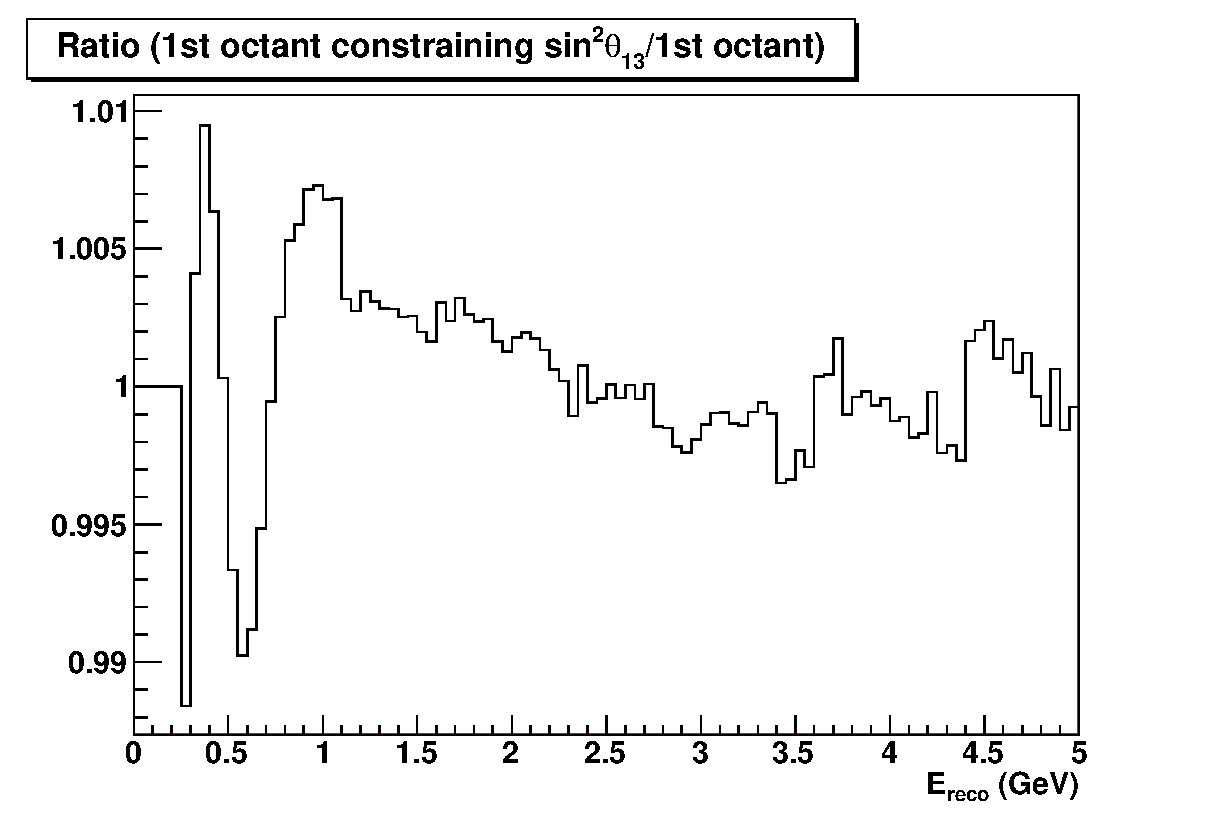
\includegraphics[width=0.5\textwidth]{images/validation/ExampleDistributionFirstOctantConstrainRatio.eps}
%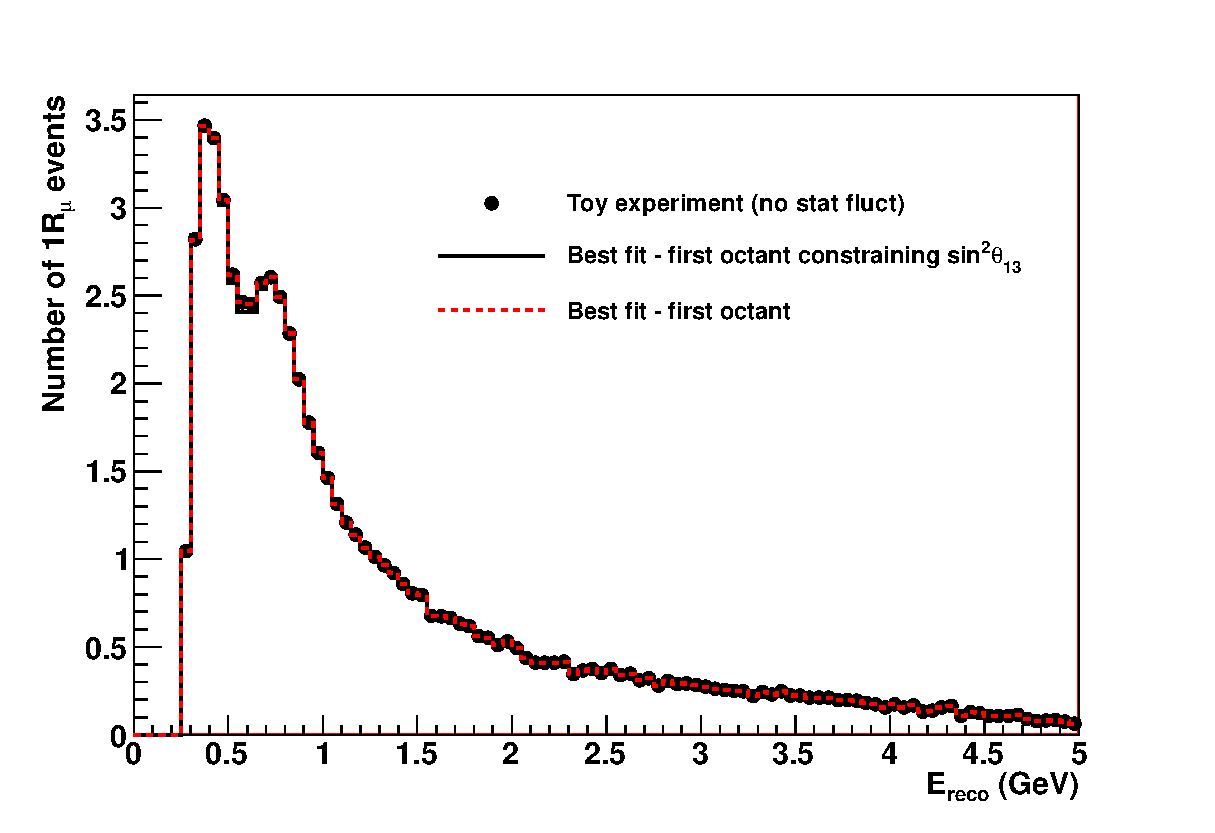
\includegraphics[width=0.5\textwidth]{images/validation/ExampleDistributionFirstOctantConstrainCurrent.eps}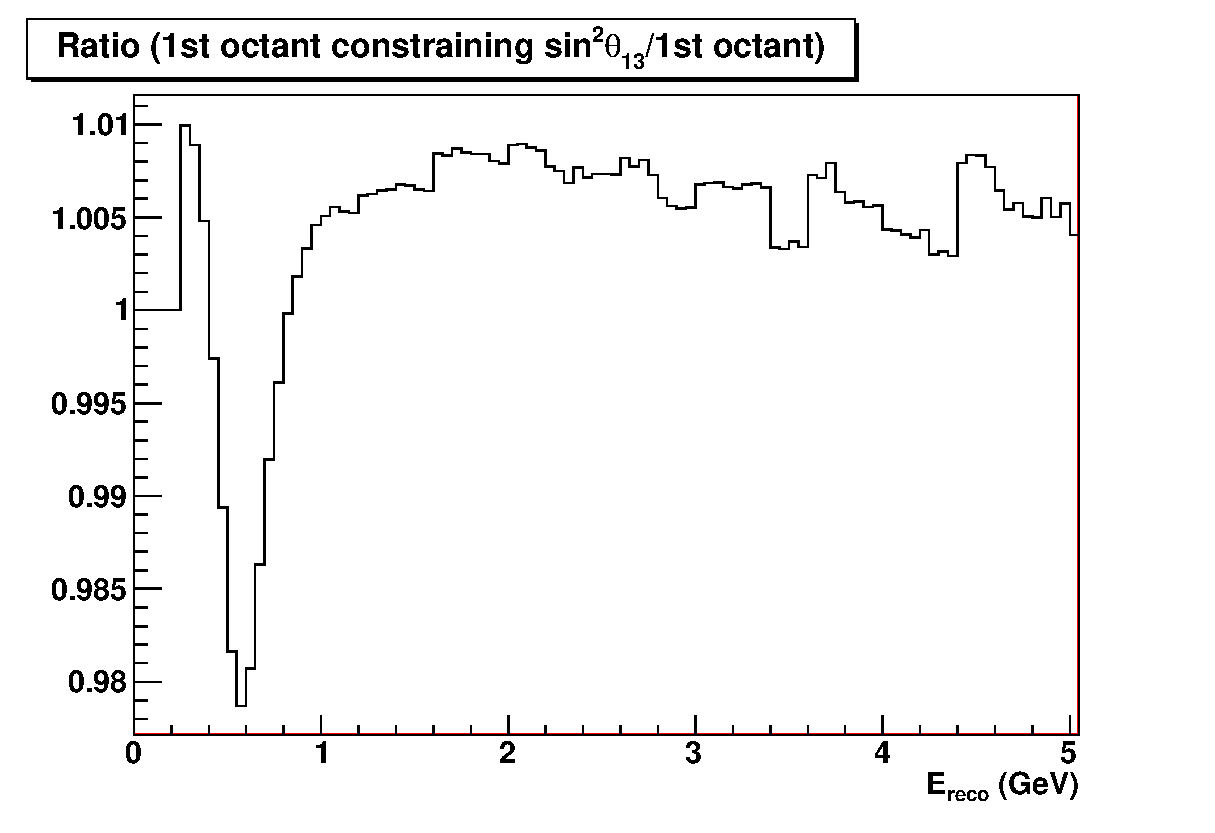
\includegraphics[width=0.5\textwidth]{images/validation/ExampleDistributionFirstOctantConstrainRatioCurrent.eps}
\caption{Best-fit reconstructed energy spectrum of one $\mu$-like ring events in the first octant for one example toy experiment with a true input value of 
$\sin^{2}\theta_{23}$ = 0.64 for the estimated final POT (7$\times$10$^{21}$) with and without the constraint on $\sin^{2}\theta_{13}$ (left); ratio of 
best-fit reconstructed spectrum with the constraint to that without the constraint (right). The constraint was applied through the penalty term in equation 
\ref{eq:chisqtot}, setting the mean of $\sin^{2}\theta_{13}$ to 0.09 (its true input value) and its error to 20\%.}
\label{fig:rdistributionconst}
\end{center}
\end{figure}

\begin{table}[h]
\centering
\begin{tabular}{|c|c|c|c|}
\hline
 & Total 1 $\mu$-like ring events & Total 1 e-like ring events\\
\hline \hline
Toy experiment & 1607.7 & 272.3 \\
Best fit, \textit{mirror} octant, without constraint on $\sin^{2}\theta_{13}$ & 1607.7 & 272.3 \\
Best fit, \textit{mirror} octant, with constraint on $\sin^{2}\theta_{13}$ & 1609.6 & 269.0\\
\hline
\end{tabular}
\caption{Best-fit numbers of one $\mu$-like ring and one e-like ring events with and without the constraint on the fitted value of $\sin^{2}\theta_{13}$; the constraint 
was applied through the penalty term in equation \ref{eq:chisqtot}, setting the mean of $\sin^{2}\theta_{13}$ to 0.09 (its true input value) and its error to 20\%.}
\label{tab:effconst}
\end{table}

The distributions of fitter residuals for $\delta_{CP}$ and $\Delta m_{32}^{2}$ were unchanged when using the mixing angles in the form $\sin^{2}\theta_{ij}$, and were 
similar to those in figures \ref{fig:res2theta} and \ref{fig:res2thetacurroth}. 

Finally, the distributions of fitted values for the different systematic parameters is presented in figure \ref{fig:systfit} for one example set of oscillation 
parameters: $\sin^{2}2\theta_{23}$ = 0.96, $|\Delta m_{32}^{2}|$ = 2.4$\times$10$^{-3}$ eV$^{2}$/c$^{4}$, $\sin^{2}2\theta_{13}$ = 0.09 and $\delta_{CP}$ = 0.

\begin{figure}[htbp]
\begin{center}
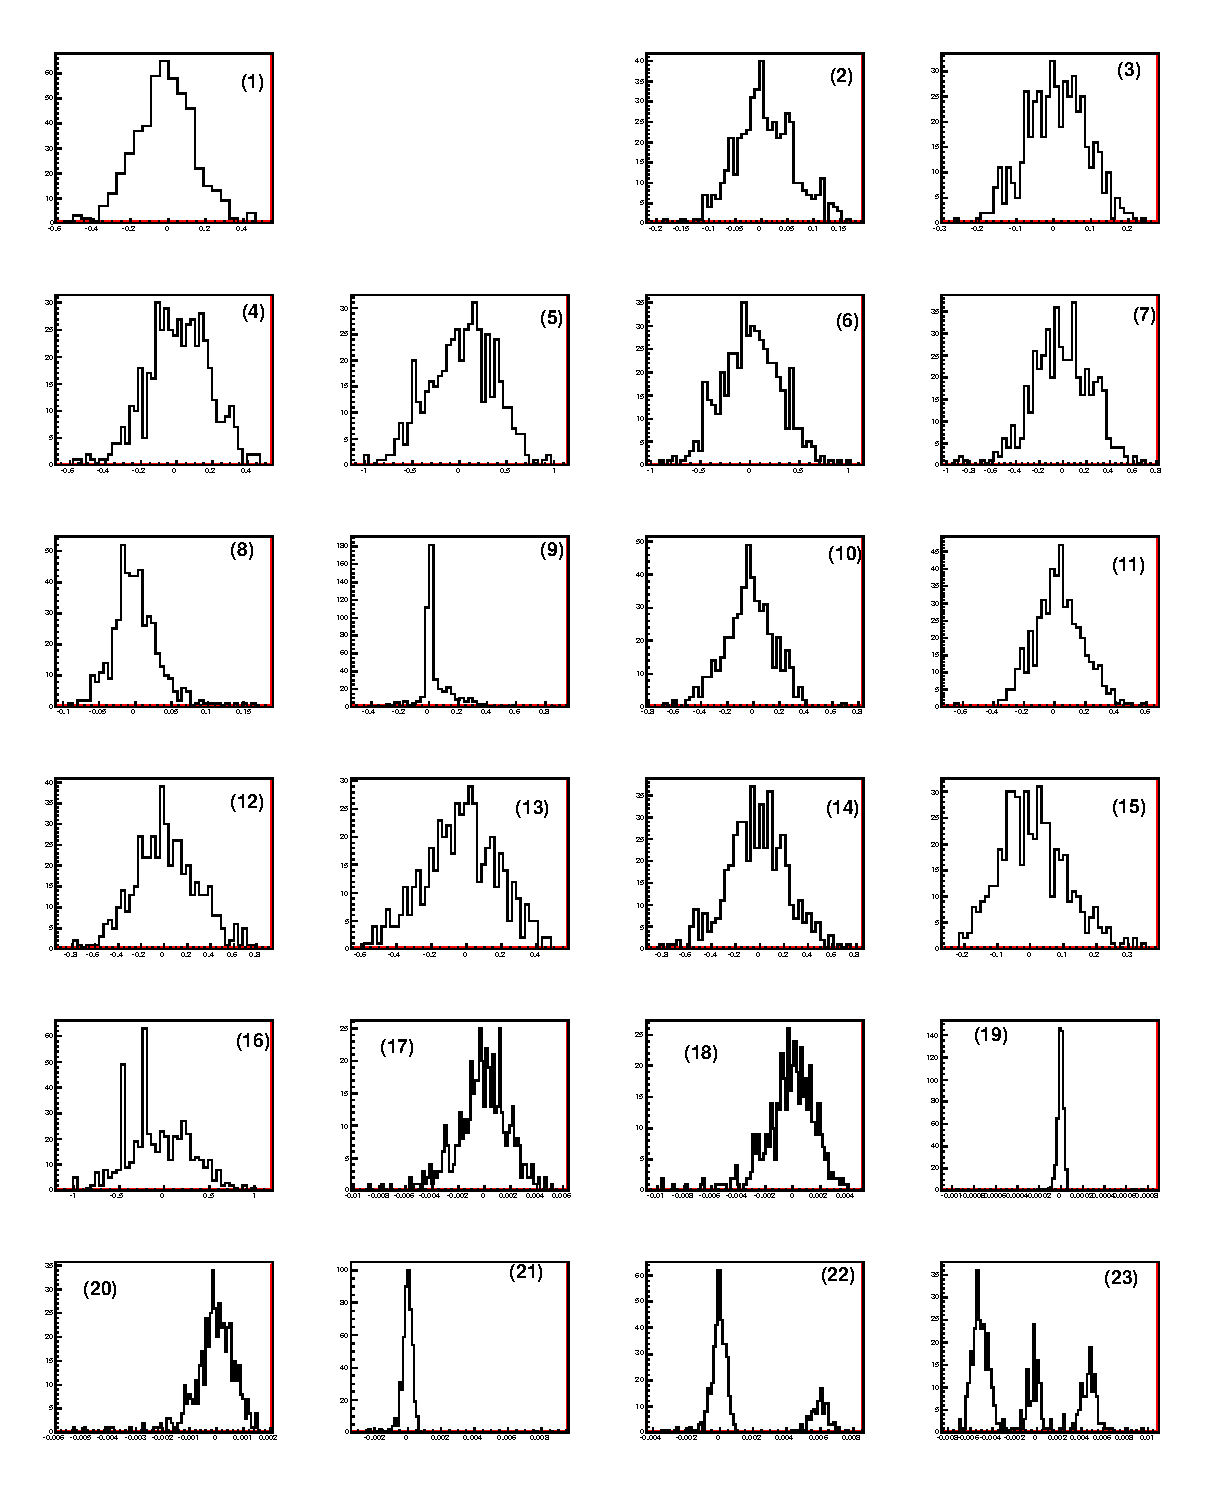
\includegraphics[width=1.0\textwidth]{images/validation/ExampleResidualsSystematics.eps}
\caption{Distributions of fitted values of the different systematic parameters for the estimated final POT (7$\times$10$^{21}$) and for one example set 
of oscillation parameters: $\sin^{2}2\theta_{23}$ = 0.96, $|\Delta m_{32}^{2}|$ = 2.4$\times$10$^{-3}$ eV$^{2}$/c$^{4}$, $\sin^{2}2\theta_{13}$ = 0.09 and $\delta_{CP}$ = 0.
The systematics are (1) Flux shape, (2) 1R$_{\mu}$ CCQE efficiency, (3), (4) and (5) 1R$_{\mu}$ CCQE ring counting efficiency, (6) 1R$_{\mu}$ CC non QE efficiency, 
(7) 1R$_{\mu}$ NC efficiency, (8) 1R$_{\mu}$ $\nu_{e}$ CC efficiency, (9) Energy scale, (10) ND280 efficiency,  (11) Flux normalization, (12) CCQE cross section, 
(13) CC1$\pi$ to CCQE cross section, (14) CC other to CCQE cross section, (15) NC to CCQE cross section, (16) Nuclear Effect, (17) 1R$_{e}$ signal efficiency, 
(18) 1R$_{e}$ background efficiency, (19) CC coh to CCQE efficiency, (20) NC 1$\pi$0 to CCQE cross section, (21) NC coh to CCQE cross section, 
(22) NC other to CCQE cross section, (23) $\nu_{e}$ to $\nu_{\mu}$ cross section. }
\label{fig:systfit}
\end{center}
\end{figure}


